\chapter{求解优化问题}

\section{拉格朗日乘子(Lagrange multipliers)}

意大利-法国数学家拉格朗日(Giuseppe Lodovico Lagrangia),也被称为约瑟夫-路易斯拉格朗日(Joseph-Louis Lagrange),发明了一种寻找受等式约束的函数的局部极大值和极小值的策略。它被称为拉格朗日乘数法

\subsection{拉格朗日乘数法}

拉格朗日注意到,当我们试图解决如下一个优化问题:
\begin{gather*}
\begin{align*}
\underset{\mathbf{x}}{\text{minimize}} \quad &f(\mathbf{x}) \\
subject\ to\quad & g(\mathbf{x})=0
\end{align*}
\end{gather*}
当 $f$的梯度点与$g$的梯度方向相同时,$f$取得最小值。 换句话说,当
\begin{gather*}
\nabla f(\mathbf{x}) = \alpha \nabla g(\mathbf{x})
\end{gather*}
所以如果我们想找到在约束$g$下的最小值$f$,我们只需要求解:
\begin{gather*}
\nabla f(\mathbf{x}) - \alpha \nabla g(\mathbf{x}) = 0
\end{gather*}

这里的常数$\alpha$也被称为拉格朗日乘子。

为了简化,我们观察到,如果我们定义一个函数$\mathcal{L}(\mathbf{x},\alpha)=f(\mathbf{x})-\alpha g(\mathbf{x})$,那么它的梯度是$\nabla\mathcal{L}(\mathbf{x},\alpha)=\nabla f(\mathbf{x})-\alpha \nabla g(\mathbf{x})$。因此,求解$\nabla\mathcal{L}(\mathbf{x},\alpha)=0$可以让我们找到最小值。


拉格朗日乘子方法可以概括为这三个步骤:
\begin{enumerate}
    \item 过为每个约束引入一个乘数来构造拉格朗日函数$\mathcal{L}$
    \item 得到拉格朗日量$\nabla \mathcal{L}$的梯度
    \item 求解$\nabla\mathcal{L}(\mathbf{x},\alpha)=0$
\end{enumerate}

\subsection{支持向量机拉格朗日问题}

上一章中提到SVM的优化问题为:
\begin{gather*}
\begin{align*}
\underset{\mathbf{w},b}{\text{minimize}} \quad &\frac{1}{2}\|w\|^2 \\
subject\ to\quad &y_i(\mathbf{w}\cdot\mathbf{x}_i+b) \geq 1,i=1,\dots,m
\end{align*}
\end{gather*}

让我们回 到这个问题,我们需要最小化一个目标函数:
\begin{gather*}
f(\mathbf{w}) = \frac{1}{2}\|w\|^2
\end{gather*}
和$m$个约束函数:
\begin{gather*}
g_i(\mathbf{w},b)=y_i(\mathbf{w}\cdot \mathbf{x}_i+b)-1,i=1,\dots,m
\end{gather*}
我们引入拉格朗日函数:
\begin{gather*}
\mathcal{L}(\mathbf{w},b,a)=f(\mathbf{w})\sum_{i=1}^m \alpha_i g_i(\mathbf{w},b) \\
\mathcal{L}(\mathbf{w},b,a)=\frac{1}{2}\|\mathbf{w}\|^2-\sum_{i=1}^m \alpha_i [y_i(\mathbf{w}\cdot \mathbf{x}_i)+b-1]
\end{gather*}
注意,我们为每个约束函数引入了一个拉格朗日乘子$\alpha_i$

我们可以试着求解$\mathcal{L}(\mathbf{w},b,a)=0$,但这个问题只能在样本数量较少的情况下用分析的方法解决(Tyson Smith, 2004)。我们再一次用对偶原理重写这个问题。

为了得到原问题的解,我们需要解下面的拉格朗日问题:
\begin{gather*}
\begin{align*}
\min_{\mathbf{w},b} \max_\alpha \quad &\mathcal{L}(\mathbf{w},b,a) \\
subject\ to\quad &\alpha_i \geq 0,i=1,dots,m
\end{align*}
\end{gather*}

这里有趣的是我们需要在$\mathbf{w}$和$b$的情况下最小化,同时在$\alpha$的情况下最大化

> tip:你们可能已经注意到拉格朗日乘数法是用来解决等式约束的问题的,而这里我们用的是不等式约束的问题。这是因为,如果满足一些附加条件(KKT条件),该方法仍然适用于不等式约束。我们稍后将讨论这些条件。



\section{对偶问题(The wolfe dual problem)}

拉格朗日问题有$m$个不等式约束(其中$m$是训练样本的数量),通常用它的对偶形式来解决。对偶原理告诉我们,一个优化问题可以从两个角度来看。第一个是原始问题,在我们的例子中是一个最小化问题,另一个是对偶问题,也就是一个最大化问题。有趣的是对偶问题的最大值总是小于或等于原始问题的最小值(我们说它提供了原始问题解的下界)。

在我们的例子中,我们试图解决一个凸优化问题,而\textbf{Slater条件}适用于仿射约束(Gretton, 2016),所以\textbf{Slater定理}告诉我们\textbf{强对偶性}成立。这意味着对偶问题的最大值等于原始问题的最小值。解对偶和解原函数是一样的,只是它更简单一些。

回想一下,拉格朗日函数是:
\begin{gather*}
\begin{align*}
\mathcal{L}(\mathbf{w},b,a) &= \frac{1}{2}\|\mathbf{w}\|^2-\sum_{i=1}^m \alpha_i [y_i(\mathbf{w}\cdot \mathbf{x}_i)+b-1] \\
&= \frac{1}{2}\mathbf{w} \cdot \mathbf{w}-\sum_{i=1}^m \alpha_i [y_i(\mathbf{w}\cdot \mathbf{x}_i)+b-1]
\end{align*}
\end{gather*}

拉格朗日原始问题是:
\begin{gather*}
\begin{align*}
\min_{\mathbf{w},b} \max_\alpha \quad &\mathcal{L}(\mathbf{w},b,a) \\
subject\ to\quad &\alpha_i \geq 0,i=1,dots,m
\end{align*}
\end{gather*}
求解最小化问题涉及对$\mathcal{L}$求$\mathbf{w}$和$b$的偏导数。

\begin{gather*}
\nabla_\mathbf{w} \mathcal{L} = \mathbf{w} - \sum_{i=1}^m \alpha_i y_i \mathbf{x}_i = 0 \\
\frac{\partial \mathcal{L}}{\partial b}=-\sum_{i=1}^m\alpha_i y_i = 0
\end{gather*}

从上面第一个式子中可得:
\begin{gather*}
\mathbf{w} = \sum_{i=1}^m \alpha_i y_i \mathbf{x}_i
\end{gather*}

再把$\mathbf{w}$的值代入$\mathcal{L}$:
\begin{gather*}
\begin{align*}
W(\alpha,b) &=\frac{1}{2}(\sum_{i=1}^m \alpha_i y_i \mathbf{x}_i) \cdot (\sum_{j=1}^m \alpha_j y_j \mathbf{x}_j) - \sum_{i=1}^m \alpha_i[y_i ((\sum_{j=1}^m \alpha_j y_j \mathbf{x}_j)\cdot \mathbf{x}_i+b)-1] \\
&= \frac{1}{2}\sum_{i=1}^m\sum_{j=1}^m \alpha_i \alpha_j y_i y_j \mathbf{x}_i \cdot \mathbf{x}_j - \sum_{i=1}^m\alpha_i y_i ((\sum_{j=1}^m \alpha_j y_j \mathbf{x}_j)\cdot \mathbf{x}_i+b) + \sum_{i=1}^m \alpha_i \\
&= \frac{1}{2}\sum_{i=1}^m\sum_{j=1}^m \alpha_i \alpha_j y_i y_j \mathbf{x}_i \cdot \mathbf{x}_j -\sum_{i=1}^m\sum_{j=1}^m \alpha_i \alpha_j y_i y_j \mathbf{x}_i \cdot \mathbf{x}_j - b\sum_{i=1}^m \alpha_i y_i + \sum_{i=1}^m \alpha_i \\
&= \sum_{i=1}^m \alpha_i - \frac{1}{2}\sum_{i=1}^m\sum_{j=1}^m \alpha_i \alpha_j y_i y_j \mathbf{x}_i \cdot \mathbf{x}_j  - b\sum_{i=1}^m \alpha_i y_i
\end{align*}
\end{gather*}

所以我们成功地消去了$\mathbf{w}$,但仍然在函数的最后一项中使用了$b$:
\begin{gather*}
W(\alpha,b) = \sum_{i=1}^m \alpha_i - \frac{1}{2}\sum_{i=1}^m\sum_{j=1}^m \alpha_i \alpha_j y_i y_j \mathbf{x}_i \cdot \mathbf{x}_j  - b\sum_{i=1}^m \alpha_i y_i
\end{gather*}

我们还注意到$\frac{\partial \mathcal{L}}{\partial b}= 0$,这意为着$\sum\limits_{i=1}^m\alpha_i y_i = 0$,也就是说上面的公式中最后一项为0,所以上面的式子可以写作:
\begin{gather*}
W(\alpha) = \sum_{i=1}^m \alpha_i - \frac{1}{2}\sum_{i=1}^m\sum_{j=1}^m \alpha_i \alpha_j y_i y_j \mathbf{x}_i \cdot \mathbf{x}_j 
\end{gather*}
这就是对偶拉格朗日函数

优化问题现在称为对偶问题:
\begin{gather*}
\begin{align*}
\underset{\alpha}{\text{maximize}}\quad & \sum_{i=1}^m \alpha_i - \frac{1}{2}\sum_{i=1}^m\sum_{j=1}^m \alpha_i \alpha_j y_i y_j \mathbf{x}_i \cdot \mathbf{x}_j \\
subject\ to \quad& \alpha_i \geq 0,\text{for any }i=1,\dots,m \\
 &\sum_{i=1}^m\alpha_i y_i = 0
\end{align*}
\end{gather*}

传统的对偶拉格朗日问题是受梯度为零的约束。理论上,我们应该添加约束$\nabla_\mathbf{w}\mathcal{L}$和$\frac{\partial \mathcal{L}}{\partial b}= 0$。然而,我们只添加了后者。事实上,我们增加了$\sum\limits_{i=1}^m\alpha_i y_i = 0$,因为从函数中移去$b$是必要的。然而,我们可以在没有约束$\mathbf{w}=\sum\limits_{i=1}^m \alpha_i y_i \mathbf{x}_i$的情况下解决这个问题。

对偶问题相对于拉格朗日问题的主要优点是目标函数$W$现在只依赖于拉格朗日乘子。此外,这个公式将在下一节中帮助我们在Python中解决这个问题,并且在我们稍后定义核时将非常有用。

\section{KKT条件(Karush-Kuhn-Tucker conditions)}
由于我们处理的是不等式约束,因此有一个额外的要求:解必须也满足Karush-Kuhn-Tucker (KKT)条件

KKT条件是优化问题解是最优解的一阶必要条件。此外,该问题还应满足一定的正则性条件。幸运的是,其中一个正则性条件是Slater条件,我们刚刚看到它适用于支持向量机。由于我们试图解决的原问题是一个凸问题,KKT也是原问题和对偶问题最优解的充分条件,且这两个解是没有对偶间隙(duality gap)的。

\textbf{综上所述,如果一个解满足KKT条件,我们可以保证它是最优解}

KKT条件有:

* 固定条件(Stationarity):
\begin{gather*}
\nabla_\mathbf{w} \mathcal{L} = \mathbf{w} - \sum_{i=1}^m \alpha_i y_i \mathbf{x}_i = 0 \\
\frac{\partial \mathcal{L}}{\partial b}=-\sum_{i=1}^m\alpha_i y_i = 0
\end{gather*}
* 原始的可行性条件(Primal feasibility)
\begin{gather*}
y_i (\mathbf{w} \cdot \mathbf{x}_i + b) -1 \geq 0 \qquad \text{for all }i=1,\dots,m
\end{gather*}

* 对偶可行性条件(Dual feasibility)
\begin{gather*}
\alpha_i \geq 0 \qquad \text{for all }i=1,\dots,m
\end{gather*}

* 松弛互补条件(Complementary slackness)
\begin{gather*}
\alpha_i[y_i (\mathbf{w} \cdot \mathbf{x}_i + b) -1] =0 \qquad \text{for all }i=1,\dots,m
\end{gather*}

> Note: "求解支持向量机问题相当于求解KKT条件"(Burges, 1988)

请注意,我们之前已经看到了其中的大多数条件。让我们逐一检查一下。

\subsection{ 固定条件(Stationarity)}
固定条件告诉我们所选的点必须是一个静止点。它是函数停止递增或递减的点。当无约束条件时,固定条件为目标函数的梯度为零的点。当我们有约束条件时,我们使用拉格朗日函数的梯度。

\subsection{原始的可行性条件}

观察这个条件,你应该认识到原始问题的约束条件。为了在约束下找到函数的最小值,它们必须被强制执行,这是有道理的

\subsection{对偶可行性条件}

同样,这个条件表示对偶问题必须遵守的约束条件。

\subsection{松弛互补条件}

从松弛互补条件中很明显可以得出$\alpha_i=0$或$y_i (\mathbf{w} \cdot \mathbf{x}_i + b) -1=0$

\textbf{支持向量}是具有正拉格朗日乘子的样本,它们也都满足$y_i (\mathbf{w} \cdot \mathbf{x}_i + b) -1 \geq 0$这个约束条件。(这也意味着对支持向量来说$y_i (\mathbf{w} \cdot \mathbf{x}_i + b) -1=0$)

> Tip:从互补松弛条件可以看出,支持向量是具有正拉格朗日乘子的样本。

\section{有了乘子之后该怎么做?}

当我们解决对偶问题时,我们得到一个包含所有拉格朗日乘子的向量$\alpha$。然而,当我们最初陈述原始问题时,我们的目标是找到$\mathbf{w}$和$b$。让我们看看如何从拉格朗日乘数中得到这些值。

\subsection{计算$\mathbf{W}$}

从之前的公式$\nabla_\mathbf{w} \mathcal{L}$中,我们很容易得到$\mathbf{w} = \sum\limits_{i=1}^m \alpha_i y_i \mathbf{x}_i$


\subsection{计算$b$}
当有了$\mathbf{w}$后,我们可以用原始问题的约束条件来计算$b$:
\begin{gather*}
y_i (\mathbf{w} \cdot \mathbf{x}_i + b) -1 \geq 0
\end{gather*}
事实上,这个约束仍然成立,因为我们将原来的问题转化成新的公式是等价的。它的意思是,离超平面最近的点的函数间隔为1(这个1是我们利用缩放所选择的值):
\begin{gather*}
y_i (\mathbf{w} \cdot \mathbf{x}_i + b) = 1
\end{gather*}

我们知道上面公式中的所有其他变量,很容易求出$b$。等式两边同时乘以$y_i$,因为$y_i^2=1$(记住$y_i$只有$+1,-1$两个取值),得到:
\begin{gather*}
\mathbf{w} \cdot \mathbf{x}_i + b = y_i \\
b = y_i - \mathbf{w} \cdot \mathbf{x}_i
\end{gather*}

然而,正如在《模式识别与机器学习》(Pattern Recognition and Machine Learning. Bishop, 2006)中指出的那样,取平均值,而不是随机的支持向量$\mathbf{x}_i$,可以为我们提供一个数值上更稳定的解:
\begin{gather*}
b = \frac{1}{S} \sum_{i=1}^S(y_i - \mathbf{w} \cdot \mathbf{x}_i)
\end{gather*}
其中$S$是支持向量的数量。

其他作者,如(Cristianini \& shaw - taylor, 2000)和(Ng),使用的是另一个公式:
\begin{gather*}
b = - \frac{\max_{y_i=-1}(\mathbf{w} \cdot \mathbf{x}_i)+\min_{y_i=1}(\mathbf{w} \cdot \mathbf{x}_i)}{2}
\end{gather*}

它们取最近的正支持向量和最近的负支持向量的平均值。这个最新的公式最初是由统计学习理论(Vapnik V. N., 1998)在定义最优超平面时使用的。

\subsection{假设函数(Hypothesis function)}

支持向量机使用与感知机相同的假设函数。一个样本的类别由以下给出:
\begin{gather*}
h(\mathbf{x}_i) = sign(\mathbf{w} \cdot \mathbf{x}_i+b)
\end{gather*}

当使用对偶公式时,仅使用支持向量来计算:
\begin{gather*}
h(\mathbf{x}_i) = sign(\sum_{j=1}^S \alpha_j y_j (\mathbf{x}_j \cdot \mathbf{x}_i)+b)
\end{gather*}


\section{用QP求解器求解支持向量机}

QP求解器是一种用于求解二次规划问题的程序。在下面的例子中,我们将使用名为\href{http://cvxopt.org/}{CVXOPT}的Python包。

这个包提供了一种方法,能够解决如下形式的二次问题:
\begin{gather*}
\begin{align*}
\underset{x}{\text{minimize}} \quad & \frac{1}{2}x^T P x+q^T x \\
subject\ to \quad &Gx \preceq h \\
& Ax = b
\end{align*}
\end{gather*}

它看起来不像我们的优化问题,所以我们需要重写它,以便我们可以用这个包来解决它。

首先,我们注意到在对偶优化问题的情况下,我们试图最小化的是$\alpha$,所以我们可以用$\alpha$代替$x$重写二次问题,来更好地看两个问题是如何关联的:
\begin{gather*}
\begin{align*}
\underset{x}{\text{minimize}} \quad & \frac{1}{2}\alpha^T P \alpha+q^T \alpha \\
subject\ to \quad &G \alpha \preceq h \\
& A \alpha = b
\end{align*}
\end{gather*}

这里的$\preceq$符号表示逐分量向量不等式(component-wise vector ineqalities)。它意味着矩阵$G \lambda$的每一行都代表一个必须满足的不等式。

我们要改变对偶问题。首先,我们将最大化问题转化为:
\begin{gather*}
\begin{align*}
\underset{\alpha}{\text{maximize}} \quad & - \frac{1}{2}\sum_{i=1}^m\sum_{j=1}^m \alpha_i \alpha_j y_i y_j \mathbf{x}_i \cdot \mathbf{x}_j + \sum_{i=1}^m \alpha_i \\
subject\ to \quad & \alpha_i \geq 0,\text{for any }i=1,\dots,m \\
& \sum_{i=1}^m \alpha_i y_i = 0
\end{align*}
\end{gather*}

乘以-1变为最小化问题:
\begin{gather*}
\begin{align*}
\underset{\alpha}{\text{minimize}} \quad & \frac{1}{2}\sum_{i=1}^m\sum_{j=1}^m \alpha_i \alpha_j y_i y_j \mathbf{x}_i \cdot \mathbf{x}_j - \sum_{i=1}^m \alpha_i \\
subject\ to \quad & -\alpha_i \geq 0,\text{for any }i=1,\dots,m \\
& \sum_{i=1}^m \alpha_i y_i = 0
\end{align*}
\end{gather*}

然后我们引入向量$\alpha = (\alpha_1,dots,\alpha_m)^T$和$y = (y_1,\dots,y_m)^T$以及所有可能的向量$x_i$的点积的Gram矩阵$K$:
\begin{gather*}
K(\mathbf{x}_1,\dots,\mathbf{x}_m) = 
\begin{pmatrix}
\mathbf{x}_1 \cdot \mathbf{x}_1 & \mathbf{x}_1 \cdot \mathbf{x}_2 &\dots &\mathbf{x}_1 \cdot \mathbf{x}_m \\
\mathbf{x}_2 \cdot \mathbf{x}_1 & \mathbf{x}_2 \cdot \mathbf{x}_2 &\dots &\mathbf{x}_2 \cdot \mathbf{x}_m \\
\vdots & \vdots & \ddots & \vdots \\
\mathbf{x}_m \cdot \mathbf{x}_1 & \mathbf{x}_m \cdot \mathbf{x}_2 &\dots &\mathbf{x}_m \cdot \mathbf{x}_m 
\end{pmatrix}
\end{gather*}

我们用它们来构造对偶问题的一个向量化版本,其中$yy^T$表示的是的$y$外积。
\begin{gather*}
\begin{align*}
\underset{x}{\text{minimize}} \quad & \frac{1}{2}\alpha^T (yy^TK) \alpha - \alpha \\
subject\ to \quad & -\alpha \preceq 0 \\
& y \alpha = 0
\end{align*}
\end{gather*}

现在,我们可以找出CVXOPT的qp函数所需的每个参数$P,q,G,h,A$以及$b$的值。代码24演示了这一点。

\emph{代码24}

\begin{lstlisting}[language=python]
# See Appendix A for more information about the dataset 
from succinctly.datasets import get_dataset, linearly_separable as ls
import cvxopt.solvers 

X, y = get_dataset(ls.get_training_examples) 
m = X.shape[0] 

# Gram matrix - The matrix of all possible inner products of X. 
K = np.array([np.dot(X[i], X[j]) for j in range(m) for i in range(m)]).reshape((m, m)) 

P = cvxopt.matrix(np.outer(y, y) * K) 
q = cvxopt.matrix(-1 * np.ones(m)) 

# Equality constraints
A = cvxopt.matrix(y, (1, m)) 
b = cvxopt.matrix(0.0) 

# Inequality constraints 
G = cvxopt.matrix(np.diag(-1 * np.ones(m))) 
h = cvxopt.matrix(np.zeros(m)) 

# Solve the problem 
solution = cvxopt.solvers.qp(P, q, G, h, A, b) 

# Lagrange multipliers 
multipliers = np.ravel(solution['x']) 

# Support vectors have positive multipliers. 
has_positive_multiplier = multipliers > 1e-7 
sv_multipliers = multipliers[has_positive_multiplier] 

support_vectors = X[has_positive_multiplier] 
support_vectors_y = y[has_positive_multiplier]

\end{lstlisting}

代码24初始化所有必需的参数,并将它们传递给qp函数,qp函数返回一个解。解包含很多元素,但我们只关心$x$,在我们的例子中,它对应于拉格朗日乘数。

正如我们之前看到的,我们可以用所有的拉格朗日乘数重新计算$\mathbf{w}$:$\mathbf{w}=\sum\limits_{i=1}^m \alpha_i y_i \mathbf{x}_i$。代码25显示了计算$\mathbf{w}$的函数的代码。

\emph{代码25}
\begin{lstlisting}[language=python]
def compute_w(multipliers, X, y): 
    return np.sum(multipliers[i] * y[i] * X[i] for i in range(len(y)))

\end{lstlisting}

因为非支持向量的拉格朗日乘数几乎为零,所以我们也可以只使用支持向量数据和它们的乘数来计算$\mathbf{w}$,如代码26所示。


\emph{代码26}
\begin{lstlisting}[language=python]
w = compute_w(multipliers, X, y) 
w_from_sv = compute_w(sv_multipliers, support_vectors, support_vectors_y) 

print(w) # [0.44444446 1.11111114] 
print(w_from_sv) # [0.44444453 1.11111128]

\end{lstlisting}

之后我们用平均法计算$b$:

\emph{代码27}
\begin{lstlisting}[language=python]
def compute_b(w, X, y): 
    return np.sum([y[i] - np.dot(w, X[i]) for i in range(len(X))])/len(X)

\end{lstlisting}

\emph{代码28}
\begin{lstlisting}[language=python]
b = compute_b(w, support_vectors, support_vectors_y) # -9.666668268506335
\end{lstlisting}

当我们在图\ref{figure32}中绘制结果时,可以看到超平面是最优超平面。与感知器相反,SVM总是返回相同的结果

\begin{figure}[ht]
	\centering
	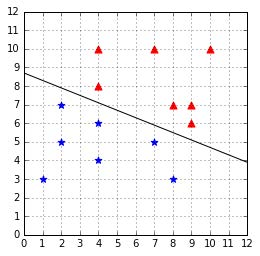
\includegraphics{figure32}
	\caption{用CVXOPT 得到的超平面}
	\label{figure32}
\end{figure}

这种支持向量机的公式称为\textbf{硬间隔支持向量机}。它不能用于数据不是线性可分的情况。支持向量机有几种公式。在下一章中,我们将考虑另一个称为\textbf{软间隔支持向量机}的公式,因为野值(outliers),它能用于数据是线性不可分的情况。


\section{总结}

$\mathbf{w}$模的最小化是一个\textbf{凸优化问题},可以用拉格朗日乘数法求解。当有更多的样本时,我们更喜欢使用凸优化包,它将为我们完成所有困难的工作。

我们看到原来的优化问题可以用拉格朗日函数重写。然后,借助于对偶理论,我们将拉格朗日问题转化为对偶问题。我们最终使用CVXOPT包来解决对偶问题。